Jedním ze zkoušených způsobů vícevláknového výpočtu problému \textit{MBP} byl \textit{task paralelismus} s pomocí knihovny \textit{OpenMP}.
Task paralelismus jsem řešil obalování značné části kódu v rekurzivní funkci jako \verb|omp task|.
Task byl přidělen jinému vláknu, každé 15 zanoření, aby nevznikala zbytečně velká režie.

U paralelizace obecně bylo důležité zajistit, aby se počítač vyvaroval časově závislým chybám.
Proto se sekce, kde se přepisuje dosavadní maximu zaobalila jako kritická sekce.
To se provedlo pomocí příkazu \verb|#pragma omp critical|.

Velkým zlepšením mé implementace by mohlo být ukládání proměnných potřebných pro rekurzivní podinstance dynamicky. To by umožnilo zbavení se nutnosti \verb|#pragma omp taskwait|.
Dalším zlepšením mé implementace by mohlo být experimentování s nastavovanou hodnotou a jejím optimálním nastavením.
Posledních \textit{n} zanoření by také mohlo dokončit tentýž vlákno.

V následující tabulce je zachycen čas výpočtu na instancích v závislosti na přidělených jádrech.
Byly použiti stejné instance, jako při sekvenčním řešení.

\FloatBarrier
\begin{table}[]
    \begin{tabular}{l|rrr}
                    instance &    čas (s) &  počet vláken &  počet procesů \\
    \hline
    graf\_15\_8.txt & 185.194 &           2 &         1 \\
    graf\_15\_8.txt & 119.916 &           4 &         1 \\
    graf\_15\_8.txt & 152.628 &           8 &         1 \\
    graf\_15\_8.txt & 300.773 &          16 &         1 \\
    graf\_15\_8.txt & 384.658 &          20 &         1 \\
    graf\_18\_7.txt & 380.512 &           2 &         1 \\
    graf\_18\_7.txt & 234.348 &           4 &         1 \\
    graf\_18\_7.txt & 290.757 &           8 &         1 \\
    graf\_21\_6.txt & 172.210 &           2 &         1 \\
    graf\_21\_6.txt & 113.647 &           4 &         1 \\
    graf\_21\_6.txt & 136.511 &           8 &         1 \\
    graf\_21\_6.txt & 275.099 &          16 &         1 \\
    graf\_21\_6.txt & 345.112 &          20 &         1 \\
    \end{tabular}
\end{table}

\FloatBarrier

Pro lepší přehlednost jsem zobrazil výpočetní čas na grafu.


\begin{figure}[!htbp]
\centerline{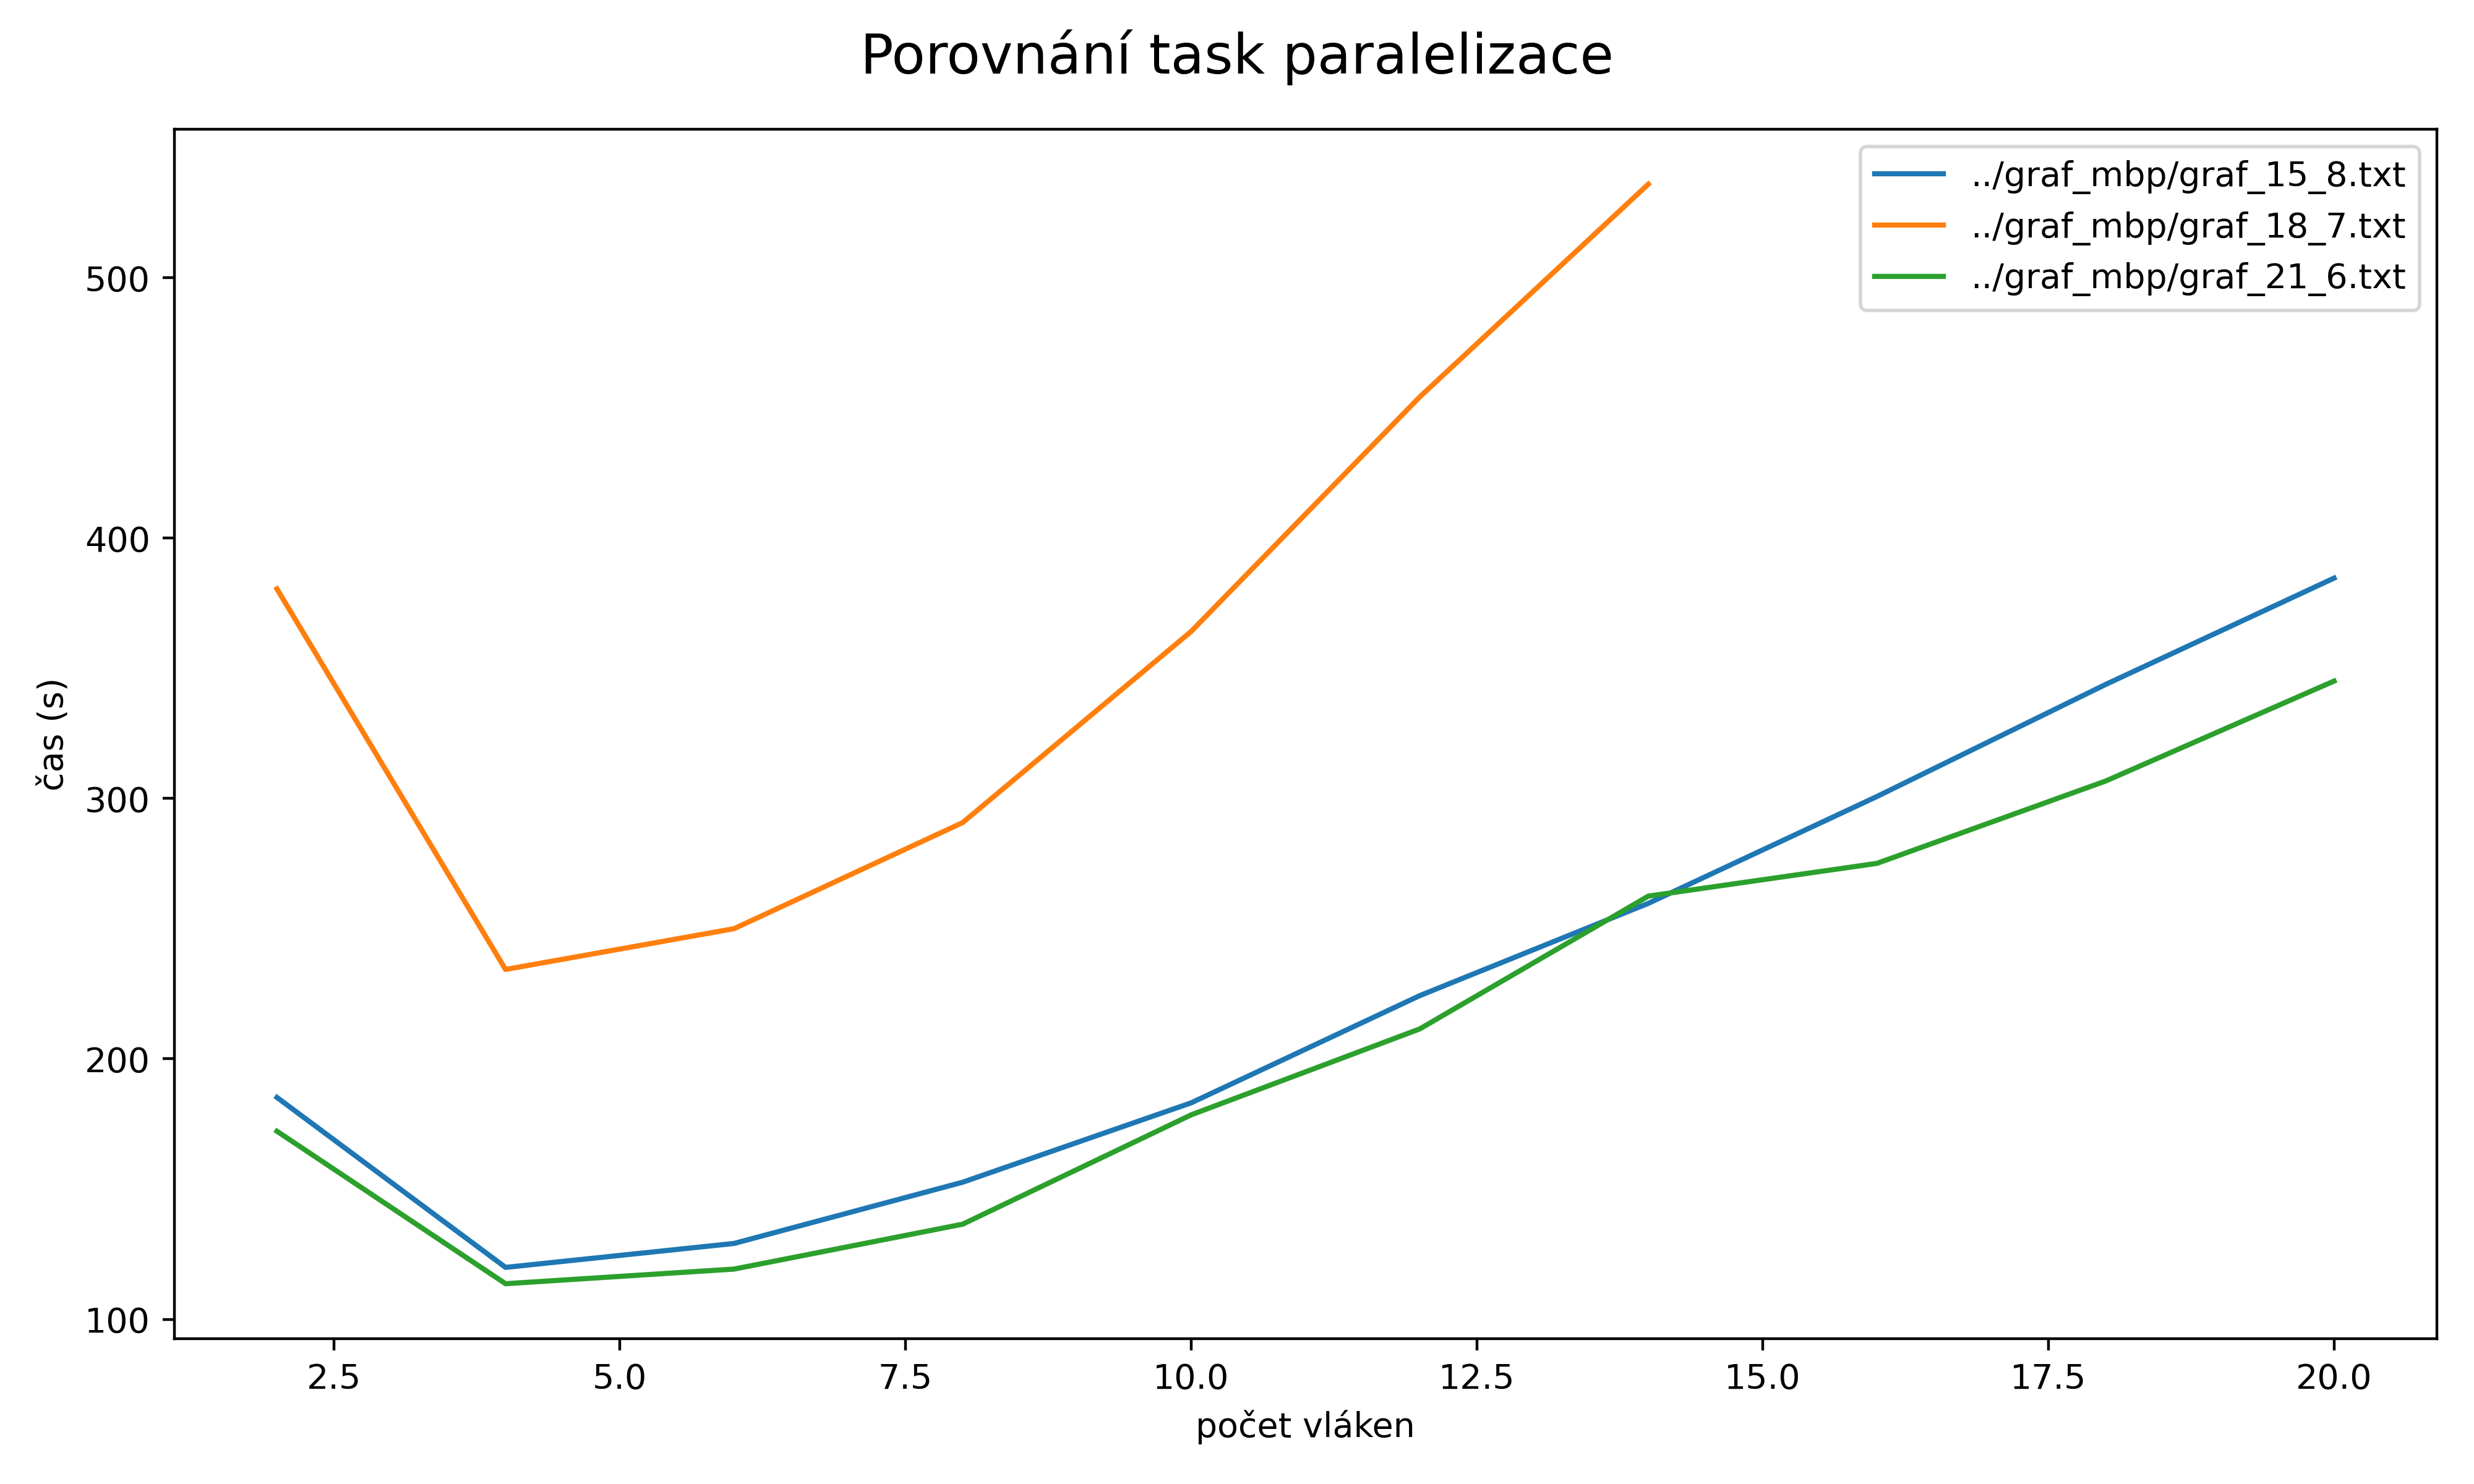
\includegraphics[scale=.46]{images/porovnání_task_paralelizace.png}}
\caption{Škálování OpenMP task paralelizace}
\end{figure}

\FloatBarrier

Z výsledků je zjevné, že režie v tomto typu paralelismu vyžaduje příliš.
